
\documentclass[xcolor={dvipsnames}]{beamer}
\usepackage{amsmath,amsfonts,amssymb,pxfonts,eulervm,xspace}
\usepackage{graphicx}
 \usepackage{multimedia}
\usepackage{media9}
\usepackage{minted}
\usepackage{mathtools}

\usepackage{animate}

\graphicspath{{./figures/}}
\usetheme{ccnycrest}


\begin{document}

\title{ CS102: Introduction to Classes}
\author{Hannah Aizenman}


\begin{frame}
	\titlepage
\end{frame}

\begin{frame}{P1}
	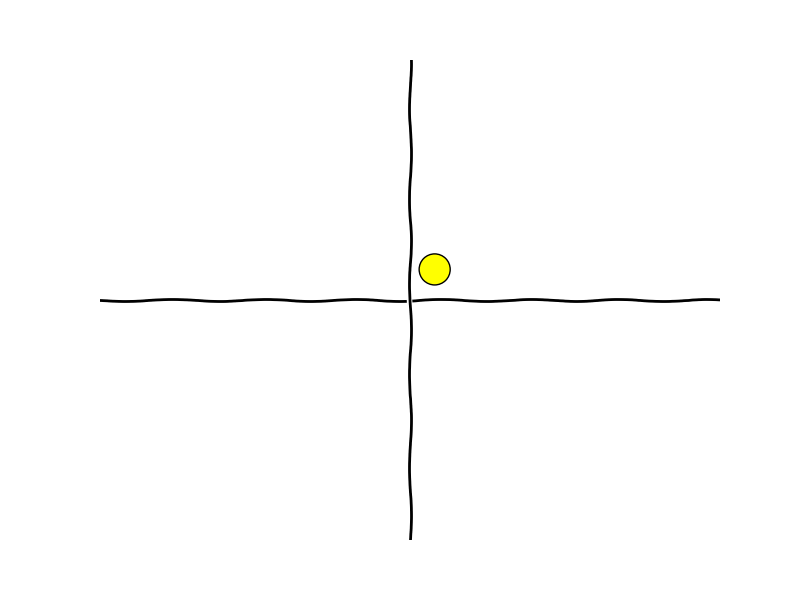
\includegraphics[width=1\textwidth]{traj000}
\end{frame}

\begin{frame}[fragile]{Point Structs}
\begin{block}{Create Struct Object Type}
\begin{minted}{c++}
struct Point{
    int x;
    int y;
    std::string color;
};
\end{minted}
\end{block}

\begin{block}{Use Struct Object Type}
\begin{minted}{c++}
Point p = {1, 2, "yellow"};
cout<<p.x<<" "<<p.y<<endl;
\end{minted}
\end{block}
\end{frame}

\begin{frame}[fragile]{Structs: Functions}
\begin{block}{Struct as Argument}
\begin{minted}{c++}
void display(Point p){ cout<<p.x<<" "<<p.y<<endl; }
\end{minted}
\end{block}
\begin{block}{Pointer to Struct as Argument}
\begin{minted}{c++}
int distance(Point *p1, Point *p2){
    return sqrt((pow(p1->x,2.0)-pow(p2->x, 2.0))+
                (pow(p1->y,2.0) - pow(p2->y, 2.0)));
}
\end{minted}
\begin{block}{Calling Function with struct}
\begin{minted}{c++}
display(p);
distance(&p, &p2);
\end{minted}
\end{block}
\end{block}
\end{frame}

\begin{frame}[fragile]{Point Object}
\begin{block}{Declaration: Describe the Point}
\begin{minted}{c++}
class Point{
    public:
        int x;
        int y;
        std::string color;
        Point(int nx, int ny, std::string c);
}
\end{minted}
\end{block}
\pause
\begin{block}{Constructor: Create the Point}
\begin{minted}{c++}
Point::Point(int nx, int ny, std::string c){
    x = nx;
    y = ny;
    color = c;
}
\end{minted}
\end{block}
\end{frame}

\begin{frame}[fragile]{Work with an Instance of the Point Class: P1}
\begin{minted}{c++}
#include <iostream>
#include <string>
#include "point.h"

using namespace std;
int main(){
    //create point
    string color = "yellow";
    Point p1(0,0, color);
    cout<<p1.x<<" "<<p1.y<<endl;
    return 0;
}
\end{minted}
\end{frame}

\begin{frame}{P1 Moves}
	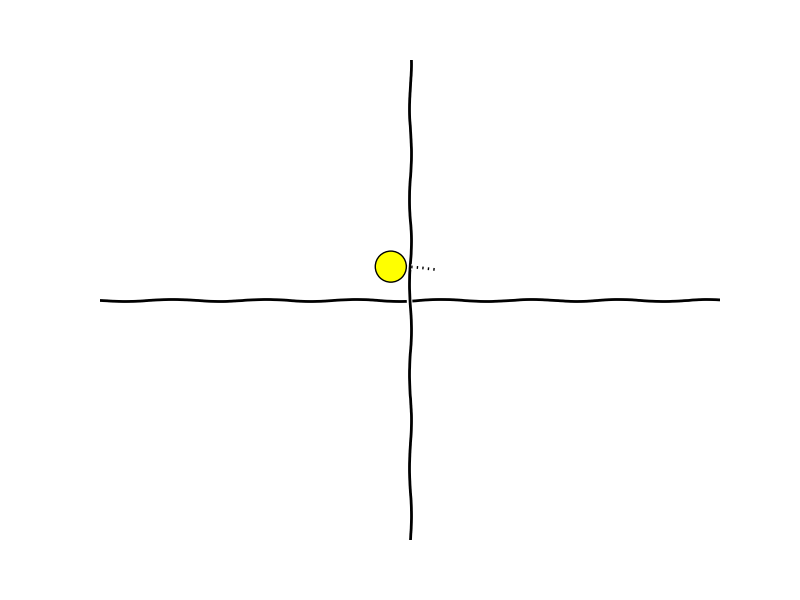
\includegraphics[width=1\textwidth]{traj001}
\end{frame}

\begin{frame}[fragile]{Move a Point}
\begin{minted}{c++}
void Point::move(int nx, int ny){
    x+=nx;
    y+=ny;
}
\end{minted}
\end{frame}

\begin{frame}[fragile]{Update the Point Declaration}
\begin{minted}{c++}
class Point{
    public:
        int x;
        int y;
        std::string color;
        Point(int nx, int nx, std::string c);
        void move(int nx, int ny);
};
\end{minted}
\end{frame}


\begin{frame}[fragile]{Move P1}
\begin{minted}{c++}
int main(){
    //create point
    string color = "yellow";
    Point p1(0,0, color);
    p1.move(1,1);
    cout<<p1.x<<" "<<p1.y<<endl;
    p1.move(-2, 0);
    cout<<p1.x<<" "<<p1.y<<endl;
    return 0;
}
\end{minted}
\end{frame}


\begin{frame}[fragile]{Working with Multiple Instances: P1, P2}
\begin{minted}{c++}
int main(){
    //create point
    string color = "yellow";
    Point p1(0,0, color);
    cout<<p1.x<<" "<<p1.y<<endl;
   //create second point
   Point p2(1,1, "blue");
   cout<<p2.x<<" "<<p2.y<<endl;
   return 0;
}
\end{minted}
\end{frame}

\begin{frame}[fragile]{Compare Two Points: Object as Argument}
\begin{minted}{c++}
bool Point::equal(Point P){
    return ((x==P.x)&&(y==P.y));
}
\end{minted}
\end{frame}

\begin{frame}[fragile]{Update the Point Declaration}
\begin{minted}{c++}
class Point{
    public:
        int x;
        int y;
        std::string color;
        Point(int x0, int y0, std::string c0);
        void move(int nx, int ny);
        bool equal(Point P);
};
\end{minted}
\end{frame}

\begin{frame}[fragile]{Compare P1 and P2}
\begin{minted}{c++}
int main(){
    //create point
    string color = "yellow";
    Point p1(0,0, color);
    cout<<p1.x<<" "<<p1.y<<endl;
    //create second point
    Point p2(1,1, "blue");
    cout<<p2.x<<" "<<p2.y<<endl;
    cout<<"Equal? "<<p1.equal(p2)<<endl;
    return 0;
}
\end{minted}
\end{frame}
\end{document}

